\documentclass[1p]{elsarticle_modified}
%\bibliographystyle{elsarticle-num}

%\usepackage[colorlinks]{hyperref}
%\usepackage{abbrmath_seonhwa} %\Abb, \Ascr, \Acal ,\Abf, \Afrak
\usepackage{amsfonts}
\usepackage{amssymb}
\usepackage{amsmath}
\usepackage{amsthm}
\usepackage{scalefnt}
\usepackage{amsbsy}
\usepackage{kotex}
\usepackage{caption}
\usepackage{subfig}
\usepackage{color}
\usepackage{graphicx}
\usepackage{xcolor} %% white, black, red, green, blue, cyan, magenta, yellow
\usepackage{float}
\usepackage{setspace}
\usepackage{hyperref}

\usepackage{tikz}
\usetikzlibrary{arrows}

\usepackage{multirow}
\usepackage{array} % fixed length table
\usepackage{hhline}

%%%%%%%%%%%%%%%%%%%%%
\makeatletter
\renewcommand*\env@matrix[1][\arraystretch]{%
	\edef\arraystretch{#1}%
	\hskip -\arraycolsep
	\let\@ifnextchar\new@ifnextchar
	\array{*\c@MaxMatrixCols c}}
\makeatother %https://tex.stackexchange.com/questions/14071/how-can-i-increase-the-line-spacing-in-a-matrix
%%%%%%%%%%%%%%%

\usepackage[normalem]{ulem}

\newcommand{\msout}[1]{\ifmmode\text{\sout{\ensuremath{#1}}}\else\sout{#1}\fi}
%SOURCE: \msout is \stkout macro in https://tex.stackexchange.com/questions/20609/strikeout-in-math-mode

\newcommand{\cancel}[1]{
	\ifmmode
	{\color{red}\msout{#1}}
	\else
	{\color{red}\sout{#1}}
	\fi
}

\newcommand{\add}[1]{
	{\color{blue}\uwave{#1}}
}

\newcommand{\replace}[2]{
	\ifmmode
	{\color{red}\msout{#1}}{\color{blue}\uwave{#2}}
	\else
	{\color{red}\sout{#1}}{\color{blue}\uwave{#2}}
	\fi
}

\newcommand{\Sol}{\mathcal{S}} %segment
\newcommand{\D}{D} %diagram
\newcommand{\A}{\mathcal{A}} %arc


%%%%%%%%%%%%%%%%%%%%%%%%%%%%%5 test

\def\sl{\operatorname{\textup{SL}}(2,\Cbb)}
\def\psl{\operatorname{\textup{PSL}}(2,\Cbb)}
\def\quan{\mkern 1mu \triangleright \mkern 1mu}

\theoremstyle{definition}
\newtheorem{thm}{Theorem}[section]
\newtheorem{prop}[thm]{Proposition}
\newtheorem{lem}[thm]{Lemma}
\newtheorem{ques}[thm]{Question}
\newtheorem{cor}[thm]{Corollary}
\newtheorem{defn}[thm]{Definition}
\newtheorem{exam}[thm]{Example}
\newtheorem{rmk}[thm]{Remark}
\newtheorem{alg}[thm]{Algorithm}

\newcommand{\I}{\sqrt{-1}}
\begin{document}

%\begin{frontmatter}
%
%\title{Boundary parabolic representations of knots up to 8 crossings}
%
%%% Group authors per affiliation:
%\author{Yunhi Cho} 
%\address{Department of Mathematics, University of Seoul, Seoul, Korea}
%\ead{yhcho@uos.ac.kr}
%
%
%\author{Seonhwa Kim} %\fnref{s_kim}}
%\address{Center for Geometry and Physics, Institute for Basic Science, Pohang, 37673, Korea}
%\ead{ryeona17@ibs.re.kr}
%
%\author{Hyuk Kim}
%\address{Department of Mathematical Sciences, Seoul National University, Seoul 08826, Korea}
%\ead{hyukkim@snu.ac.kr}
%
%\author{Seokbeom Yoon}
%\address{Department of Mathematical Sciences, Seoul National University, Seoul, 08826,  Korea}
%\ead{sbyoon15@snu.ac.kr}
%
%\begin{abstract}
%We find all boundary parabolic representation of knots up to 8 crossings.
%
%\end{abstract}
%\begin{keyword}
%    \MSC[2010] 57M25 
%\end{keyword}
%
%\end{frontmatter}

%\linenumbers
%\tableofcontents
%
\newcommand\colored[1]{\textcolor{white}{\rule[-0.35ex]{0.8em}{1.4ex}}\kern-0.8em\color{red} #1}%
%\newcommand\colored[1]{\textcolor{white}{ #1}\kern-2.17ex	\textcolor{white}{ #1}\kern-1.81ex	\textcolor{white}{ #1}\kern-2.15ex\color{red}#1	}

{\Large $\underline{12a_{0977}~(K12a_{0977})}$}

\setlength{\tabcolsep}{10pt}
\renewcommand{\arraystretch}{1.6}
\vspace{1cm}\begin{tabular}{m{100pt}>{\centering\arraybackslash}m{274pt}}
\multirow{5}{120pt}{
	\centering
	\includegraphics[width=112pt]{../../../GIT/diagram.site/Diagrams/png/1778_12a_0977.png}\\
\ \ \ A knot diagram\footnotemark}&
\allowdisplaybreaks
\textbf{Linearized knot diagam} \\
\cline{2-2}
 &
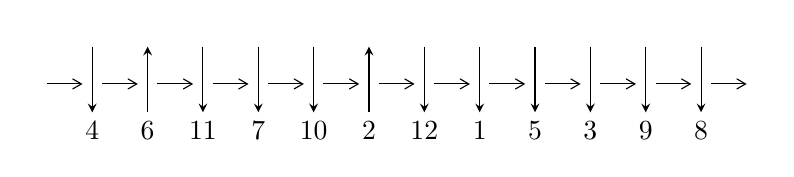
\begin{tikzpicture}[x=20pt, y=17pt]
	% nodes
	\node (C0) at (0, 0) {};
	\node (C1) at (1, 0) {};
	\node (C1U) at (1, +1) {};
	\node (C1D) at (1, -1) {4};

	\node (C2) at (2, 0) {};
	\node (C2U) at (2, +1) {};
	\node (C2D) at (2, -1) {6};

	\node (C3) at (3, 0) {};
	\node (C3U) at (3, +1) {};
	\node (C3D) at (3, -1) {11};

	\node (C4) at (4, 0) {};
	\node (C4U) at (4, +1) {};
	\node (C4D) at (4, -1) {7};

	\node (C5) at (5, 0) {};
	\node (C5U) at (5, +1) {};
	\node (C5D) at (5, -1) {10};

	\node (C6) at (6, 0) {};
	\node (C6U) at (6, +1) {};
	\node (C6D) at (6, -1) {2};

	\node (C7) at (7, 0) {};
	\node (C7U) at (7, +1) {};
	\node (C7D) at (7, -1) {12};

	\node (C8) at (8, 0) {};
	\node (C8U) at (8, +1) {};
	\node (C8D) at (8, -1) {1};

	\node (C9) at (9, 0) {};
	\node (C9U) at (9, +1) {};
	\node (C9D) at (9, -1) {5};

	\node (C10) at (10, 0) {};
	\node (C10U) at (10, +1) {};
	\node (C10D) at (10, -1) {3};

	\node (C11) at (11, 0) {};
	\node (C11U) at (11, +1) {};
	\node (C11D) at (11, -1) {9};

	\node (C12) at (12, 0) {};
	\node (C12U) at (12, +1) {};
	\node (C12D) at (12, -1) {8};
	\node (C13) at (13, 0) {};

	% arrows
	\draw[->,>={angle 60}]
	(C0) edge (C1) (C1) edge (C2) (C2) edge (C3) (C3) edge (C4) (C4) edge (C5) (C5) edge (C6) (C6) edge (C7) (C7) edge (C8) (C8) edge (C9) (C9) edge (C10) (C10) edge (C11) (C11) edge (C12) (C12) edge (C13) ;	\draw[->,>=stealth]
	(C1U) edge (C1D) (C2D) edge (C2U) (C3U) edge (C3D) (C4U) edge (C4D) (C5U) edge (C5D) (C6D) edge (C6U) (C7U) edge (C7D) (C8U) edge (C8D) (C9U) edge (C9D) (C10U) edge (C10D) (C11U) edge (C11D) (C12U) edge (C12D) ;
	\end{tikzpicture} \\
\hhline{~~} \\& 
\textbf{Solving Sequence} \\ \cline{2-2} 
 &
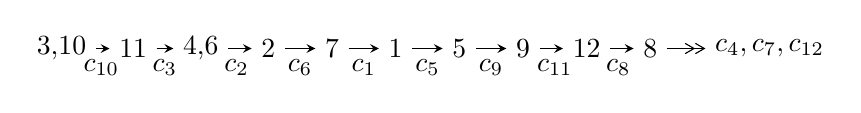
\begin{tikzpicture}[x=23pt, y=7pt]
	% node
	\node (A0) at (-1/8, 0) {3,10};
	\node (A1) at (1, 0) {11};
	\node (A2) at (33/16, 0) {4,6};
	\node (A3) at (25/8, 0) {2};
	\node (A4) at (33/8, 0) {7};
	\node (A5) at (41/8, 0) {1};
	\node (A6) at (49/8, 0) {5};
	\node (A7) at (57/8, 0) {9};
	\node (A8) at (65/8, 0) {12};
	\node (A9) at (73/8, 0) {8};
	\node (C1) at (1/2, -1) {$c_{10}$};
	\node (C2) at (3/2, -1) {$c_{3}$};
	\node (C3) at (21/8, -1) {$c_{2}$};
	\node (C4) at (29/8, -1) {$c_{6}$};
	\node (C5) at (37/8, -1) {$c_{1}$};
	\node (C6) at (45/8, -1) {$c_{5}$};
	\node (C7) at (53/8, -1) {$c_{9}$};
	\node (C8) at (61/8, -1) {$c_{11}$};
	\node (C9) at (69/8, -1) {$c_{8}$};
	\node (A10) at (11, 0) {$c_{4},c_{7},c_{12}$};

	% edge
	\draw[->,>=stealth]	
	(A0) edge (A1) (A1) edge (A2) (A2) edge (A3) (A3) edge (A4) (A4) edge (A5) (A5) edge (A6) (A6) edge (A7) (A7) edge (A8) (A8) edge (A9) ;
	\draw[->>,>={angle 60}]	
	(A9) edge (A10);
\end{tikzpicture} \\ 

\end{tabular} \\

\footnotetext{
The image of knot diagram is generated by the software ``\textbf{Draw programme}" developed by Andrew Bartholomew(\url{http://www.layer8.co.uk/maths/draw/index.htm\#Running-draw}), where we modified some parts for our purpose(\url{https://github.com/CATsTAILs/LinksPainter}).
}\phantom \\ \newline 
\centering \textbf{Ideals for irreducible components\footnotemark of $X_{\text{par}}$} 
 
\begin{align*}
I^u_{1}&=\langle 
b- u,\;-6.57813\times10^{24} u^{37}+6.93409\times10^{24} u^{36}+\cdots+1.58961\times10^{25} a-1.79176\times10^{25},\\
\phantom{I^u_{1}}&\phantom{= \langle  }u^{38}- u^{37}+\cdots-2 u-1\rangle \\
I^u_{2}&=\langle 
-3.41732\times10^{236} u^{71}-6.79357\times10^{235} u^{70}+\cdots+4.34076\times10^{236} b+1.29907\times10^{241},\\
\phantom{I^u_{2}}&\phantom{= \langle  }4.33939\times10^{191} u^{71}+8.92073\times10^{190} u^{70}+\cdots+5.46565\times10^{191} a-1.64326\times10^{196},\\
\phantom{I^u_{2}}&\phantom{= \langle  }u^{72}- u^{71}+\cdots+27418 u+45671\rangle \\
I^u_{3}&=\langle 
b+u,\;-29744507 u^{22}+20395822 u^{21}+\cdots+15493951 a-35668774,\;u^{23}- u^{22}+\cdots+2 u-1\rangle \\
\\
\end{align*}
\raggedright * 3 irreducible components of $\dim_{\mathbb{C}}=0$, with total 133 representations.\\
\footnotetext{All coefficients of polynomials are rational numbers. But the coefficients are sometimes approximated in decimal forms when there is not enough margin.}
\newpage
\renewcommand{\arraystretch}{1}
\centering \section*{I. $I^u_{1}= \langle b- u,\;-6.58\times10^{24} u^{37}+6.93\times10^{24} u^{36}+\cdots+1.59\times10^{25} a-1.79\times10^{25},\;u^{38}- u^{37}+\cdots-2 u-1 \rangle$}
\flushleft \textbf{(i) Arc colorings}\\
\begin{tabular}{m{7pt} m{180pt} m{7pt} m{180pt} }
\flushright $a_{3}=$&$\begin{pmatrix}0\\u\end{pmatrix}$ \\
\flushright $a_{10}=$&$\begin{pmatrix}1\\0\end{pmatrix}$ \\
\flushright $a_{11}=$&$\begin{pmatrix}1\\u^2\end{pmatrix}$ \\
\flushright $a_{4}=$&$\begin{pmatrix}- u\\- u^3+u\end{pmatrix}$ \\
\flushright $a_{6}=$&$\begin{pmatrix}0.413821 u^{37}-0.436214 u^{36}+\cdots-1.50019 u+1.12717\\u\end{pmatrix}$ \\
\flushright $a_{2}=$&$\begin{pmatrix}0.116083 u^{37}-0.0485543 u^{36}+\cdots-2.44812 u-1.74726\\-0.0852640 u^{37}-0.0336343 u^{36}+\cdots+0.630964 u+0.0223927\end{pmatrix}$ \\
\flushright $a_{7}=$&$\begin{pmatrix}-0.230273 u^{37}+0.259709 u^{36}+\cdots+1.51707 u+1.86697\\-0.0298691 u^{37}+0.209123 u^{36}+\cdots+0.379824 u-0.0451359\end{pmatrix}$ \\
\flushright $a_{1}=$&$\begin{pmatrix}-0.0235968 u^{37}+0.113861 u^{36}+\cdots-1.86834 u-1.50048\\0.0600474 u^{37}-0.161614 u^{36}+\cdots-0.0430228 u-0.201654\end{pmatrix}$ \\
\flushright $a_{5}=$&$\begin{pmatrix}0.413821 u^{37}-0.436214 u^{36}+\cdots-0.500191 u+1.12717\\u\end{pmatrix}$ \\
\flushright $a_{9}=$&$\begin{pmatrix}0.0223927 u^{37}-0.107657 u^{36}+\cdots-1.95481 u+0.586179\\- u^2\end{pmatrix}$ \\
\flushright $a_{12}=$&$\begin{pmatrix}-0.231100 u^{37}+0.0117291 u^{36}+\cdots+0.254712 u+1.24608\\-0.144821 u^{37}+0.0158346 u^{36}+\cdots-0.0732163 u+0.0228410\end{pmatrix}$ \\
\flushright $a_{8}=$&$\begin{pmatrix}-0.252060 u^{37}-0.112582 u^{36}+\cdots+0.324884 u+1.39835\\-0.124431 u^{37}+0.0520392 u^{36}+\cdots-0.454891 u-0.274698\end{pmatrix}$\\&\end{tabular}
\flushleft \textbf{(ii) Obstruction class $= -1$}\\~\\
\flushleft \textbf{(iii) Cusp Shapes $= \frac{30044921907723853376224412}{15896073949776978916320991} u^{37}-\frac{55405836824956460952841385}{15896073949776978916320991} u^{36}+\cdots-\frac{101017582556204696388328298}{15896073949776978916320991} u-\frac{126386542644867906673421663}{15896073949776978916320991}$}\\~\\
\newpage\renewcommand{\arraystretch}{1}
\flushleft \textbf{(iv) u-Polynomials at the component}\newline \\
\begin{tabular}{m{50pt}|m{274pt}}
Crossings & \hspace{64pt}u-Polynomials at each crossing \\
\hline $$\begin{aligned}c_{1},c_{4}\end{aligned}$$&$\begin{aligned}
&u^{38}-2 u^{37}+\cdots+4 u+1
\end{aligned}$\\
\hline $$\begin{aligned}c_{2},c_{6}\end{aligned}$$&$\begin{aligned}
&u^{38}-26 u^{37}+\cdots+65536 u-4096
\end{aligned}$\\
\hline $$\begin{aligned}c_{3},c_{5},c_{9}\\c_{10}\end{aligned}$$&$\begin{aligned}
&u^{38}- u^{37}+\cdots-2 u-1
\end{aligned}$\\
\hline $$\begin{aligned}c_{7},c_{8},c_{12}\end{aligned}$$&$\begin{aligned}
&u^{38}+9 u^{37}+\cdots-28 u+8
\end{aligned}$\\
\hline $$\begin{aligned}c_{11}\end{aligned}$$&$\begin{aligned}
&u^{38}-30 u^{37}+\cdots+43124 u-3512
\end{aligned}$\\
\hline
\end{tabular}\\~\\
\newpage\renewcommand{\arraystretch}{1}
\flushleft \textbf{(v) Riley Polynomials at the component}\newline \\
\begin{tabular}{m{50pt}|m{274pt}}
Crossings & \hspace{64pt}Riley Polynomials at each crossing \\
\hline $$\begin{aligned}c_{1},c_{4}\end{aligned}$$&$\begin{aligned}
&y^{38}-4 y^{37}+\cdots-94 y+1
\end{aligned}$\\
\hline $$\begin{aligned}c_{2},c_{6}\end{aligned}$$&$\begin{aligned}
&y^{38}+26 y^{37}+\cdots-125829120 y+16777216
\end{aligned}$\\
\hline $$\begin{aligned}c_{3},c_{5},c_{9}\\c_{10}\end{aligned}$$&$\begin{aligned}
&y^{38}-33 y^{37}+\cdots+2 y+1
\end{aligned}$\\
\hline $$\begin{aligned}c_{7},c_{8},c_{12}\end{aligned}$$&$\begin{aligned}
&y^{38}-33 y^{37}+\cdots-80 y+64
\end{aligned}$\\
\hline $$\begin{aligned}c_{11}\end{aligned}$$&$\begin{aligned}
&y^{38}+6 y^{37}+\cdots-103314128 y+12334144
\end{aligned}$\\
\hline
\end{tabular}\\~\\
\newpage\flushleft \textbf{(vi) Complex Volumes and Cusp Shapes}
$$\begin{array}{c|c|c}  
\text{Solutions to }I^u_{1}& \I (\text{vol} + \sqrt{-1}CS) & \text{Cusp shape}\\
 \hline 
\begin{aligned}
u &= -0.642582 + 0.529294 I \\
a &= -0.362091 - 0.970748 I \\
b &= -0.642582 + 0.529294 I\end{aligned}
 & -0.62981 + 3.65009 I & -8.45785 - 7.32483 I \\ \hline\begin{aligned}
u &= -0.642582 - 0.529294 I \\
a &= -0.362091 + 0.970748 I \\
b &= -0.642582 - 0.529294 I\end{aligned}
 & -0.62981 - 3.65009 I & -8.45785 + 7.32483 I \\ \hline\begin{aligned}
u &= -0.311299 + 0.761183 I \\
a &= -0.085459 - 0.793774 I \\
b &= -0.311299 + 0.761183 I\end{aligned}
 & -1.66830 - 2.81679 I & -7.20948 + 0.94774 I \\ \hline\begin{aligned}
u &= -0.311299 - 0.761183 I \\
a &= -0.085459 + 0.793774 I \\
b &= -0.311299 - 0.761183 I\end{aligned}
 & -1.66830 + 2.81679 I & -7.20948 - 0.94774 I \\ \hline\begin{aligned}
u &= -1.199830 + 0.197665 I \\
a &= -0.39774 - 1.71231 I \\
b &= -1.199830 + 0.197665 I\end{aligned}
 & -5.74703 + 1.70191 I & -30.1093 - 4.4341 I \\ \hline\begin{aligned}
u &= -1.199830 - 0.197665 I \\
a &= -0.39774 + 1.71231 I \\
b &= -1.199830 - 0.197665 I\end{aligned}
 & -5.74703 - 1.70191 I & -30.1093 + 4.4341 I \\ \hline\begin{aligned}
u &= -1.214180 + 0.163826 I \\
a &= -1.142910 - 0.562138 I \\
b &= -1.214180 + 0.163826 I\end{aligned}
 & -3.58346 + 2.28431 I & -12.26521 - 5.93080 I \\ \hline\begin{aligned}
u &= -1.214180 - 0.163826 I \\
a &= -1.142910 + 0.562138 I \\
b &= -1.214180 - 0.163826 I\end{aligned}
 & -3.58346 - 2.28431 I & -12.26521 + 5.93080 I \\ \hline\begin{aligned}
u &= \phantom{-}0.441998 + 0.630000 I \\
a &= \phantom{-}0.143471 - 0.902436 I \\
b &= \phantom{-}0.441998 + 0.630000 I\end{aligned}
 & \phantom{-}2.72467 - 0.41534 I & -1.86874 + 2.50646 I \\ \hline\begin{aligned}
u &= \phantom{-}0.441998 - 0.630000 I \\
a &= \phantom{-}0.143471 + 0.902436 I \\
b &= \phantom{-}0.441998 - 0.630000 I\end{aligned}
 & \phantom{-}2.72467 + 0.41534 I & -1.86874 - 2.50646 I\\
 \hline 
 \end{array}$$\newpage$$\begin{array}{c|c|c}  
\text{Solutions to }I^u_{1}& \I (\text{vol} + \sqrt{-1}CS) & \text{Cusp shape}\\
 \hline 
\begin{aligned}
u &= \phantom{-}0.125697 + 0.754675 I \\
a &= \phantom{-}1.46136 - 0.33666 I \\
b &= \phantom{-}0.125697 + 0.754675 I\end{aligned}
 & -4.16749 + 6.80742 I & -11.39539 - 4.57055 I \\ \hline\begin{aligned}
u &= \phantom{-}0.125697 - 0.754675 I \\
a &= \phantom{-}1.46136 + 0.33666 I \\
b &= \phantom{-}0.125697 - 0.754675 I\end{aligned}
 & -4.16749 - 6.80742 I & -11.39539 + 4.57055 I \\ \hline\begin{aligned}
u &= \phantom{-}0.319015 + 0.661353 I \\
a &= -1.13060 - 0.90619 I \\
b &= \phantom{-}0.319015 + 0.661353 I\end{aligned}
 & -5.30082 + 0.18015 I & -13.27778 + 1.55316 I \\ \hline\begin{aligned}
u &= \phantom{-}0.319015 - 0.661353 I \\
a &= -1.13060 + 0.90619 I \\
b &= \phantom{-}0.319015 - 0.661353 I\end{aligned}
 & -5.30082 - 0.18015 I & -13.27778 - 1.55316 I \\ \hline\begin{aligned}
u &= \phantom{-}1.262990 + 0.084911 I \\
a &= \phantom{-}0.66371 - 1.32119 I \\
b &= \phantom{-}1.262990 + 0.084911 I\end{aligned}
 & -11.45280 + 3.42761 I & -20.1823 - 6.5471 I \\ \hline\begin{aligned}
u &= \phantom{-}1.262990 - 0.084911 I \\
a &= \phantom{-}0.66371 + 1.32119 I \\
b &= \phantom{-}1.262990 - 0.084911 I\end{aligned}
 & -11.45280 - 3.42761 I & -20.1823 + 6.5471 I \\ \hline\begin{aligned}
u &= \phantom{-}1.263310 + 0.274194 I \\
a &= \phantom{-}0.921270 - 0.499067 I \\
b &= \phantom{-}1.263310 + 0.274194 I\end{aligned}
 & -2.35527 - 7.30757 I & -10.63293 + 7.72113 I \\ \hline\begin{aligned}
u &= \phantom{-}1.263310 - 0.274194 I \\
a &= \phantom{-}0.921270 + 0.499067 I \\
b &= \phantom{-}1.263310 - 0.274194 I\end{aligned}
 & -2.35527 + 7.30757 I & -10.63293 - 7.72113 I \\ \hline\begin{aligned}
u &= \phantom{-}1.255600 + 0.363345 I \\
a &= -0.019509 - 1.407240 I \\
b &= \phantom{-}1.255600 + 0.363345 I\end{aligned}
 & -8.61451 - 7.26588 I & -15.9503 + 10.7715 I \\ \hline\begin{aligned}
u &= \phantom{-}1.255600 - 0.363345 I \\
a &= -0.019509 + 1.407240 I \\
b &= \phantom{-}1.255600 - 0.363345 I\end{aligned}
 & -8.61451 + 7.26588 I & -15.9503 - 10.7715 I\\
 \hline 
 \end{array}$$\newpage$$\begin{array}{c|c|c}  
\text{Solutions to }I^u_{1}& \I (\text{vol} + \sqrt{-1}CS) & \text{Cusp shape}\\
 \hline 
\begin{aligned}
u &= \phantom{-}1.33470\phantom{ +0.000000I} \\
a &= \phantom{-}1.18898\phantom{ +0.000000I} \\
b &= \phantom{-}1.33470\phantom{ +0.000000I}\end{aligned}
 & -12.3935\phantom{ +0.000000I} & -21.7990\phantom{ +0.000000I} \\ \hline\begin{aligned}
u &= -1.335100 + 0.309048 I \\
a &= -0.853516 - 0.422112 I \\
b &= -1.335100 + 0.309048 I\end{aligned}
 & -8.15095 + 11.42250 I & -14.3546 - 7.5460 I \\ \hline\begin{aligned}
u &= -1.335100 - 0.309048 I \\
a &= -0.853516 + 0.422112 I \\
b &= -1.335100 - 0.309048 I\end{aligned}
 & -8.15095 - 11.42250 I & -14.3546 + 7.5460 I \\ \hline\begin{aligned}
u &= -0.170696 + 0.593684 I \\
a &= -1.78466 - 0.26897 I \\
b &= -0.170696 + 0.593684 I\end{aligned}
 & \phantom{-}0.71316 - 3.70227 I & -4.70598 + 2.17127 I \\ \hline\begin{aligned}
u &= -0.170696 - 0.593684 I \\
a &= -1.78466 + 0.26897 I \\
b &= -0.170696 - 0.593684 I\end{aligned}
 & \phantom{-}0.71316 + 3.70227 I & -4.70598 - 2.17127 I \\ \hline\begin{aligned}
u &= \phantom{-}0.441678 + 0.391338 I \\
a &= \phantom{-}1.83459 + 0.60874 I \\
b &= \phantom{-}0.441678 + 0.391338 I\end{aligned}
 & -2.20747 + 1.18529 I & -14.4340 + 4.4751 I \\ \hline\begin{aligned}
u &= \phantom{-}0.441678 - 0.391338 I \\
a &= \phantom{-}1.83459 - 0.60874 I \\
b &= \phantom{-}0.441678 - 0.391338 I\end{aligned}
 & -2.20747 - 1.18529 I & -14.4340 - 4.4751 I \\ \hline\begin{aligned}
u &= -1.50663 + 0.36313 I \\
a &= -0.112277 - 1.068330 I \\
b &= -1.50663 + 0.36313 I\end{aligned}
 & -17.9039 + 7.3787 I & \phantom{-0.000000 } 0 \\ \hline\begin{aligned}
u &= -1.50663 - 0.36313 I \\
a &= -0.112277 + 1.068330 I \\
b &= -1.50663 - 0.36313 I\end{aligned}
 & -17.9039 - 7.3787 I & \phantom{-0.000000 } 0 \\ \hline\begin{aligned}
u &= \phantom{-}1.46940 + 0.49385 I \\
a &= -0.023597 - 1.058640 I \\
b &= \phantom{-}1.46940 + 0.49385 I\end{aligned}
 & -10.00620 - 8.86952 I & \phantom{-0.000000 } 0\\
 \hline 
 \end{array}$$\newpage$$\begin{array}{c|c|c}  
\text{Solutions to }I^u_{1}& \I (\text{vol} + \sqrt{-1}CS) & \text{Cusp shape}\\
 \hline 
\begin{aligned}
u &= \phantom{-}1.46940 - 0.49385 I \\
a &= -0.023597 + 1.058640 I \\
b &= \phantom{-}1.46940 - 0.49385 I\end{aligned}
 & -10.00620 + 8.86952 I & \phantom{-0.000000 } 0 \\ \hline\begin{aligned}
u &= -0.207067 + 0.387382 I \\
a &= \phantom{-}1.30451 - 1.62960 I \\
b &= -0.207067 + 0.387382 I\end{aligned}
 & -0.46850 + 1.50335 I & -4.10768 - 5.04879 I \\ \hline\begin{aligned}
u &= -0.207067 - 0.387382 I \\
a &= \phantom{-}1.30451 + 1.62960 I \\
b &= -0.207067 - 0.387382 I\end{aligned}
 & -0.46850 - 1.50335 I & -4.10768 + 5.04879 I \\ \hline\begin{aligned}
u &= -0.415323\phantom{ +0.000000I} \\
a &= \phantom{-}0.953137\phantom{ +0.000000I} \\
b &= -0.415323\phantom{ +0.000000I}\end{aligned}
 & -0.837431\phantom{ +0.000000I} & -10.5390\phantom{ +0.000000I} \\ \hline\begin{aligned}
u &= -1.52626 + 0.54197 I \\
a &= \phantom{-}0.036058 - 0.993072 I \\
b &= -1.52626 + 0.54197 I\end{aligned}
 & -8.3844 + 13.5000 I & \phantom{-0.000000 } 0 \\ \hline\begin{aligned}
u &= -1.52626 - 0.54197 I \\
a &= \phantom{-}0.036058 + 0.993072 I \\
b &= -1.52626 - 0.54197 I\end{aligned}
 & -8.3844 - 13.5000 I & \phantom{-0.000000 } 0 \\ \hline\begin{aligned}
u &= \phantom{-}1.57427 + 0.55070 I \\
a &= -0.023672 - 0.956443 I \\
b &= \phantom{-}1.57427 + 0.55070 I\end{aligned}
 & -13.9247 - 17.5662 I & \phantom{-0.000000 } 0 \\ \hline\begin{aligned}
u &= \phantom{-}1.57427 - 0.55070 I \\
a &= -0.023672 + 0.956443 I \\
b &= \phantom{-}1.57427 - 0.55070 I\end{aligned}
 & -13.9247 + 17.5662 I & \phantom{-0.000000 } 0\\
 \hline 
 \end{array}$$\newpage\newpage\renewcommand{\arraystretch}{1}
\centering \section*{II. $I^u_{2}= \langle -3.42\times10^{236} u^{71}-6.79\times10^{235} u^{70}+\cdots+4.34\times10^{236} b+1.30\times10^{241},\;4.34\times10^{191} u^{71}+8.92\times10^{190} u^{70}+\cdots+5.47\times10^{191} a-1.64\times10^{196},\;u^{72}- u^{71}+\cdots+27418 u+45671 \rangle$}
\flushleft \textbf{(i) Arc colorings}\\
\begin{tabular}{m{7pt} m{180pt} m{7pt} m{180pt} }
\flushright $a_{3}=$&$\begin{pmatrix}0\\u\end{pmatrix}$ \\
\flushright $a_{10}=$&$\begin{pmatrix}1\\0\end{pmatrix}$ \\
\flushright $a_{11}=$&$\begin{pmatrix}1\\u^2\end{pmatrix}$ \\
\flushright $a_{4}=$&$\begin{pmatrix}- u\\- u^3+u\end{pmatrix}$ \\
\flushright $a_{6}=$&$\begin{pmatrix}-0.793938 u^{71}-0.163215 u^{70}+\cdots+42952.0 u+30065.3\\0.787262 u^{71}+0.156506 u^{70}+\cdots-42815.4 u-29927.2\end{pmatrix}$ \\
\flushright $a_{2}=$&$\begin{pmatrix}-0.408138 u^{71}-0.0889949 u^{70}+\cdots+21707.3 u+15292.2\\0.267218 u^{71}+0.0807519 u^{70}+\cdots-12557.3 u-9274.97\end{pmatrix}$ \\
\flushright $a_{7}=$&$\begin{pmatrix}0.385823 u^{71}+0.0741978 u^{70}+\cdots-21244.3 u-14772.5\\0.617782 u^{71}+0.138655 u^{70}+\cdots-32712.3 u-23063.8\end{pmatrix}$ \\
\flushright $a_{1}=$&$\begin{pmatrix}0.328655 u^{71}+0.0965080 u^{70}+\cdots-15531.5 u-11457.2\\0.679992 u^{71}+0.171566 u^{70}+\cdots-34256.0 u-24647.7\end{pmatrix}$ \\
\flushright $a_{5}=$&$\begin{pmatrix}-0.00667606 u^{71}-0.00670817 u^{70}+\cdots+136.624 u+138.090\\0.787262 u^{71}+0.156506 u^{70}+\cdots-42815.4 u-29927.2\end{pmatrix}$ \\
\flushright $a_{9}=$&$\begin{pmatrix}0.325476 u^{71}+0.0478554 u^{70}+\cdots-18634.3 u-12815.3\\0.122394 u^{71}-0.0162808 u^{70}+\cdots-9238.65 u-5826.11\end{pmatrix}$ \\
\flushright $a_{12}=$&$\begin{pmatrix}0.101849 u^{71}+0.0284827 u^{70}+\cdots-4604.86 u-3500.59\\0.256426 u^{71}+0.0412224 u^{70}+\cdots-14192.2 u-9911.86\end{pmatrix}$ \\
\flushright $a_{8}=$&$\begin{pmatrix}0.398346 u^{71}+0.0956167 u^{70}+\cdots-20161.7 u-14516.7\\0.631835 u^{71}+0.123936 u^{70}+\cdots-34126.4 u-23950.8\end{pmatrix}$\\&\end{tabular}
\flushleft \textbf{(ii) Obstruction class $= -1$}\\~\\
\flushleft \textbf{(iii) Cusp Shapes $= -2.19731 u^{71}-0.498944 u^{70}+\cdots+116066. u+81882.3$}\\~\\
\newpage\renewcommand{\arraystretch}{1}
\flushleft \textbf{(iv) u-Polynomials at the component}\newline \\
\begin{tabular}{m{50pt}|m{274pt}}
Crossings & \hspace{64pt}u-Polynomials at each crossing \\
\hline $$\begin{aligned}c_{1},c_{4}\end{aligned}$$&$\begin{aligned}
&u^{72}-13 u^{71}+\cdots-19474 u+1151
\end{aligned}$\\
\hline $$\begin{aligned}c_{2},c_{6}\end{aligned}$$&$\begin{aligned}
&(u^3+u^2+2 u+1)^{24}
\end{aligned}$\\
\hline $$\begin{aligned}c_{3},c_{5},c_{9}\\c_{10}\end{aligned}$$&$\begin{aligned}
&u^{72}- u^{71}+\cdots+27418 u+45671
\end{aligned}$\\
\hline $$\begin{aligned}c_{7},c_{8},c_{12}\end{aligned}$$&$\begin{aligned}
&(u^{12}- u^{11}-5 u^{10}+4 u^9+9 u^8-4 u^7-6 u^6-2 u^5+3 u^3+u^2+1)^6
\end{aligned}$\\
\hline $$\begin{aligned}c_{11}\end{aligned}$$&$\begin{aligned}
&(u^{12}+3 u^{11}+\cdots+4 u+1)^{6}
\end{aligned}$\\
\hline
\end{tabular}\\~\\
\newpage\renewcommand{\arraystretch}{1}
\flushleft \textbf{(v) Riley Polynomials at the component}\newline \\
\begin{tabular}{m{50pt}|m{274pt}}
Crossings & \hspace{64pt}Riley Polynomials at each crossing \\
\hline $$\begin{aligned}c_{1},c_{4}\end{aligned}$$&$\begin{aligned}
&y^{72}-17 y^{71}+\cdots-39129988 y+1324801
\end{aligned}$\\
\hline $$\begin{aligned}c_{2},c_{6}\end{aligned}$$&$\begin{aligned}
&(y^3+3 y^2+2 y-1)^{24}
\end{aligned}$\\
\hline $$\begin{aligned}c_{3},c_{5},c_{9}\\c_{10}\end{aligned}$$&$\begin{aligned}
&y^{72}-65 y^{71}+\cdots+1084775528 y+2085840241
\end{aligned}$\\
\hline $$\begin{aligned}c_{7},c_{8},c_{12}\end{aligned}$$&$\begin{aligned}
&(y^{12}-11 y^{11}+\cdots+2 y+1)^{6}
\end{aligned}$\\
\hline $$\begin{aligned}c_{11}\end{aligned}$$&$\begin{aligned}
&(y^{12}+y^{11}+\cdots-2 y+1)^{6}
\end{aligned}$\\
\hline
\end{tabular}\\~\\
\newpage\flushleft \textbf{(vi) Complex Volumes and Cusp Shapes}
$$\begin{array}{c|c|c}  
\text{Solutions to }I^u_{2}& \I (\text{vol} + \sqrt{-1}CS) & \text{Cusp shape}\\
 \hline 
\begin{aligned}
u &= \phantom{-}0.016904 + 0.938793 I \\
a &= -1.396040 + 0.203966 I \\
b &= \phantom{-}1.209300 + 0.005604 I\end{aligned}
 & -4.84384 + 2.73451 I & \phantom{-0.000000 } 0 \\ \hline\begin{aligned}
u &= \phantom{-}0.016904 - 0.938793 I \\
a &= -1.396040 - 0.203966 I \\
b &= \phantom{-}1.209300 - 0.005604 I\end{aligned}
 & -4.84384 - 2.73451 I & \phantom{-0.000000 } 0 \\ \hline\begin{aligned}
u &= \phantom{-}0.941410 + 0.511838 I \\
a &= -0.467200 + 0.254013 I \\
b &= \phantom{-}0.102703 - 0.669479 I\end{aligned}
 & \phantom{-}1.31764 - 3.88480 I & \phantom{-0.000000 } 0 \\ \hline\begin{aligned}
u &= \phantom{-}0.941410 - 0.511838 I \\
a &= -0.467200 - 0.254013 I \\
b &= \phantom{-}0.102703 + 0.669479 I\end{aligned}
 & \phantom{-}1.31764 + 3.88480 I & \phantom{-0.000000 } 0 \\ \hline\begin{aligned}
u &= \phantom{-}0.709464 + 0.503759 I \\
a &= \phantom{-}0.66819 + 1.36798 I \\
b &= -1.64033 - 0.08580 I\end{aligned}
 & -11.07400 - 2.92173 I & \phantom{-0.000000 } 0 \\ \hline\begin{aligned}
u &= \phantom{-}0.709464 - 0.503759 I \\
a &= \phantom{-}0.66819 - 1.36798 I \\
b &= -1.64033 + 0.08580 I\end{aligned}
 & -11.07400 + 2.92173 I & \phantom{-0.000000 } 0 \\ \hline\begin{aligned}
u &= -0.108050 + 1.182640 I \\
a &= -1.079650 + 0.280505 I \\
b &= \phantom{-}1.239000 - 0.126036 I\end{aligned}
 & -4.84384 + 2.92173 I & \phantom{-0.000000 } 0 \\ \hline\begin{aligned}
u &= -0.108050 - 1.182640 I \\
a &= -1.079650 - 0.280505 I \\
b &= \phantom{-}1.239000 + 0.126036 I\end{aligned}
 & -4.84384 - 2.92173 I & \phantom{-0.000000 } 0 \\ \hline\begin{aligned}
u &= -1.053450 + 0.548334 I \\
a &= \phantom{-}0.425615 + 0.221538 I \\
b &= \phantom{-}0.003969 - 0.768800 I\end{aligned}
 & -3.82135 + 7.58818 I & \phantom{-0.000000 } 0 \\ \hline\begin{aligned}
u &= -1.053450 - 0.548334 I \\
a &= \phantom{-}0.425615 - 0.221538 I \\
b &= \phantom{-}0.003969 + 0.768800 I\end{aligned}
 & -3.82135 - 7.58818 I & \phantom{-0.000000 } 0\\
 \hline 
 \end{array}$$\newpage$$\begin{array}{c|c|c}  
\text{Solutions to }I^u_{2}& \I (\text{vol} + \sqrt{-1}CS) & \text{Cusp shape}\\
 \hline 
\begin{aligned}
u &= -1.163260 + 0.267260 I \\
a &= \phantom{-}0.420845 - 1.027000 I \\
b &= -0.205919 + 0.579765 I\end{aligned}
 & -2.81995 + 1.05668 I & \phantom{-0.000000 } 0 \\ \hline\begin{aligned}
u &= -1.163260 - 0.267260 I \\
a &= \phantom{-}0.420845 + 1.027000 I \\
b &= -0.205919 - 0.579765 I\end{aligned}
 & -2.81995 - 1.05668 I & \phantom{-0.000000 } 0 \\ \hline\begin{aligned}
u &= \phantom{-}1.209300 + 0.005604 I \\
a &= -0.182860 - 1.080060 I \\
b &= \phantom{-}0.016904 + 0.938793 I\end{aligned}
 & -4.84384 + 2.73451 I & \phantom{-0.000000 } 0 \\ \hline\begin{aligned}
u &= \phantom{-}1.209300 - 0.005604 I \\
a &= -0.182860 + 1.080060 I \\
b &= \phantom{-}0.016904 - 0.938793 I\end{aligned}
 & -4.84384 - 2.73451 I & \phantom{-0.000000 } 0 \\ \hline\begin{aligned}
u &= \phantom{-}1.203930 + 0.129844 I \\
a &= -0.060845 + 1.092290 I \\
b &= -1.94643 - 0.60072 I\end{aligned}
 & -13.09790 + 1.05668 I & \phantom{-0.000000 } 0 \\ \hline\begin{aligned}
u &= \phantom{-}1.203930 - 0.129844 I \\
a &= -0.060845 - 1.092290 I \\
b &= -1.94643 + 0.60072 I\end{aligned}
 & -13.09790 - 1.05668 I & \phantom{-0.000000 } 0 \\ \hline\begin{aligned}
u &= \phantom{-}1.182150 + 0.267603 I \\
a &= -0.458540 + 0.103800 I \\
b &= -1.354490 + 0.112254 I\end{aligned}
 & -3.82135 - 1.20211 I & \phantom{-0.000000 } 0 \\ \hline\begin{aligned}
u &= \phantom{-}1.182150 - 0.267603 I \\
a &= -0.458540 - 0.103800 I \\
b &= -1.354490 - 0.112254 I\end{aligned}
 & -3.82135 + 1.20211 I & \phantom{-0.000000 } 0 \\ \hline\begin{aligned}
u &= -0.697309 + 0.362810 I \\
a &= \phantom{-}0.643103 + 0.334607 I \\
b &= -0.316643 - 0.411076 I\end{aligned}
 & -0.706253 + 0.093609 I & -8.00000 + 0. I\phantom{ +0.000000I} \\ \hline\begin{aligned}
u &= -0.697309 - 0.362810 I \\
a &= \phantom{-}0.643103 - 0.334607 I \\
b &= -0.316643 + 0.411076 I\end{aligned}
 & -0.706253 - 0.093609 I & -8.00000 + 0. I\phantom{ +0.000000I}\\
 \hline 
 \end{array}$$\newpage$$\begin{array}{c|c|c}  
\text{Solutions to }I^u_{2}& \I (\text{vol} + \sqrt{-1}CS) & \text{Cusp shape}\\
 \hline 
\begin{aligned}
u &= -1.196300 + 0.253597 I \\
a &= -0.049609 + 1.082140 I \\
b &= \phantom{-}1.77144 - 0.52507 I\end{aligned}
 & -7.95893 + 1.62601 I & \phantom{-0.000000 } 0 \\ \hline\begin{aligned}
u &= -1.196300 - 0.253597 I \\
a &= -0.049609 - 1.082140 I \\
b &= \phantom{-}1.77144 + 0.52507 I\end{aligned}
 & -7.95893 - 1.62601 I & \phantom{-0.000000 } 0 \\ \hline\begin{aligned}
u &= \phantom{-}0.003969 + 0.768800 I \\
a &= -0.003826 + 0.741188 I \\
b &= -1.053450 - 0.548334 I\end{aligned}
 & -3.82135 - 7.58818 I & -8.98049 + 5.13539 I \\ \hline\begin{aligned}
u &= \phantom{-}0.003969 - 0.768800 I \\
a &= -0.003826 - 0.741188 I \\
b &= -1.053450 + 0.548334 I\end{aligned}
 & -3.82135 + 7.58818 I & -8.98049 - 5.13539 I \\ \hline\begin{aligned}
u &= \phantom{-}1.239000 + 0.126036 I \\
a &= -0.065594 + 1.061670 I \\
b &= -0.108050 - 1.182640 I\end{aligned}
 & -4.84384 - 2.92173 I & \phantom{-0.000000 } 0 \\ \hline\begin{aligned}
u &= \phantom{-}1.239000 - 0.126036 I \\
a &= -0.065594 - 1.061670 I \\
b &= -0.108050 + 1.182640 I\end{aligned}
 & -4.84384 + 2.92173 I & \phantom{-0.000000 } 0 \\ \hline\begin{aligned}
u &= \phantom{-}1.268300 + 0.097095 I \\
a &= -0.446678 + 0.034196 I \\
b &= -0.625462 - 0.283222 I\end{aligned}
 & -6.93644 + 0.09361 I & \phantom{-0.000000 } 0 \\ \hline\begin{aligned}
u &= \phantom{-}1.268300 - 0.097095 I \\
a &= -0.446678 - 0.034196 I \\
b &= -0.625462 + 0.283222 I\end{aligned}
 & -6.93644 - 0.09361 I & \phantom{-0.000000 } 0 \\ \hline\begin{aligned}
u &= -1.264550 + 0.238133 I \\
a &= -0.023731 + 1.029210 I \\
b &= \phantom{-}0.20647 - 1.45163 I\end{aligned}
 & -2.81995 + 6.71292 I & \phantom{-0.000000 } 0 \\ \hline\begin{aligned}
u &= -1.264550 - 0.238133 I \\
a &= -0.023731 - 1.029210 I \\
b &= \phantom{-}0.20647 + 1.45163 I\end{aligned}
 & -2.81995 - 6.71292 I & \phantom{-0.000000 } 0\\
 \hline 
 \end{array}$$\newpage$$\begin{array}{c|c|c}  
\text{Solutions to }I^u_{2}& \I (\text{vol} + \sqrt{-1}CS) & \text{Cusp shape}\\
 \hline 
\begin{aligned}
u &= -0.625462 + 0.283222 I \\
a &= \phantom{-}0.756046 + 0.342354 I \\
b &= \phantom{-}1.268300 - 0.097095 I\end{aligned}
 & -6.93644 - 0.09361 I & -10.97137 - 0.76204 I \\ \hline\begin{aligned}
u &= -0.625462 - 0.283222 I \\
a &= \phantom{-}0.756046 - 0.342354 I \\
b &= \phantom{-}1.268300 + 0.097095 I\end{aligned}
 & -6.93644 + 0.09361 I & -10.97137 + 0.76204 I \\ \hline\begin{aligned}
u &= \phantom{-}0.102703 + 0.669479 I \\
a &= -0.127574 + 0.831599 I \\
b &= \phantom{-}0.941410 - 0.511838 I\end{aligned}
 & \phantom{-}1.31764 + 3.88480 I & -4.17488 - 4.17140 I \\ \hline\begin{aligned}
u &= \phantom{-}0.102703 - 0.669479 I \\
a &= -0.127574 - 0.831599 I \\
b &= \phantom{-}0.941410 + 0.511838 I\end{aligned}
 & \phantom{-}1.31764 - 3.88480 I & -4.17488 + 4.17140 I \\ \hline\begin{aligned}
u &= \phantom{-}1.295140 + 0.280941 I \\
a &= \phantom{-}0.050487 + 0.998312 I \\
b &= -0.29281 - 1.57276 I\end{aligned}
 & -7.95893 - 10.41630 I & \phantom{-0.000000 } 0 \\ \hline\begin{aligned}
u &= \phantom{-}1.295140 - 0.280941 I \\
a &= \phantom{-}0.050487 - 0.998312 I \\
b &= -0.29281 + 1.57276 I\end{aligned}
 & -7.95893 + 10.41630 I & \phantom{-0.000000 } 0 \\ \hline\begin{aligned}
u &= -1.275570 + 0.379612 I \\
a &= \phantom{-}0.410386 + 0.122131 I \\
b &= \phantom{-}1.44696 + 0.17098 I\end{aligned}
 & -8.96033 + 3.88480 I & \phantom{-0.000000 } 0 \\ \hline\begin{aligned}
u &= -1.275570 - 0.379612 I \\
a &= \phantom{-}0.410386 - 0.122131 I \\
b &= \phantom{-}1.44696 - 0.17098 I\end{aligned}
 & -8.96033 - 3.88480 I & \phantom{-0.000000 } 0 \\ \hline\begin{aligned}
u &= \phantom{-}1.271480 + 0.448451 I \\
a &= -0.472922 - 0.861251 I \\
b &= \phantom{-}0.165937 + 0.330843 I\end{aligned}
 & -7.95893 - 4.76006 I & \phantom{-0.000000 } 0 \\ \hline\begin{aligned}
u &= \phantom{-}1.271480 - 0.448451 I \\
a &= -0.472922 + 0.861251 I \\
b &= \phantom{-}0.165937 - 0.330843 I\end{aligned}
 & -7.95893 + 4.76006 I & \phantom{-0.000000 } 0\\
 \hline 
 \end{array}$$\newpage$$\begin{array}{c|c|c}  
\text{Solutions to }I^u_{2}& \I (\text{vol} + \sqrt{-1}CS) & \text{Cusp shape}\\
 \hline 
\begin{aligned}
u &= -1.354490 + 0.112254 I \\
a &= \phantom{-}0.417835 + 0.034628 I \\
b &= \phantom{-}1.182150 + 0.267603 I\end{aligned}
 & -3.82135 - 1.20211 I & \phantom{-0.000000 } 0 \\ \hline\begin{aligned}
u &= -1.354490 - 0.112254 I \\
a &= \phantom{-}0.417835 - 0.034628 I \\
b &= \phantom{-}1.182150 - 0.267603 I\end{aligned}
 & -3.82135 + 1.20211 I & \phantom{-0.000000 } 0 \\ \hline\begin{aligned}
u &= -0.205919 + 0.579765 I \\
a &= \phantom{-}2.11905 - 0.38166 I \\
b &= -1.163260 + 0.267260 I\end{aligned}
 & -2.81995 + 1.05668 I & -10.70414 - 1.19195 I \\ \hline\begin{aligned}
u &= -0.205919 - 0.579765 I \\
a &= \phantom{-}2.11905 + 0.38166 I \\
b &= -1.163260 - 0.267260 I\end{aligned}
 & -2.81995 - 1.05668 I & -10.70414 + 1.19195 I \\ \hline\begin{aligned}
u &= \phantom{-}0.906082 + 1.051410 I \\
a &= \phantom{-}0.612247 + 0.732186 I \\
b &= -1.46963 - 0.20075 I\end{aligned}
 & -11.07400 - 2.73451 I & \phantom{-0.000000 } 0 \\ \hline\begin{aligned}
u &= \phantom{-}0.906082 - 1.051410 I \\
a &= \phantom{-}0.612247 - 0.732186 I \\
b &= -1.46963 + 0.20075 I\end{aligned}
 & -11.07400 + 2.73451 I & \phantom{-0.000000 } 0 \\ \hline\begin{aligned}
u &= -1.394260 + 0.162883 I \\
a &= \phantom{-}0.044134 + 0.942674 I \\
b &= \phantom{-}1.73833 - 0.97198 I\end{aligned}
 & -13.0979 + 6.7129 I & \phantom{-0.000000 } 0 \\ \hline\begin{aligned}
u &= -1.394260 - 0.162883 I \\
a &= \phantom{-}0.044134 - 0.942674 I \\
b &= \phantom{-}1.73833 + 0.97198 I\end{aligned}
 & -13.0979 - 6.7129 I & \phantom{-0.000000 } 0 \\ \hline\begin{aligned}
u &= \phantom{-}1.392260 + 0.231638 I \\
a &= \phantom{-}0.001675 + 0.938584 I \\
b &= -1.56676 - 0.84322 I\end{aligned}
 & -7.95893 - 4.03024 I & \phantom{-0.000000 } 0 \\ \hline\begin{aligned}
u &= \phantom{-}1.392260 - 0.231638 I \\
a &= \phantom{-}0.001675 - 0.938584 I \\
b &= -1.56676 + 0.84322 I\end{aligned}
 & -7.95893 + 4.03024 I & \phantom{-0.000000 } 0\\
 \hline 
 \end{array}$$\newpage$$\begin{array}{c|c|c}  
\text{Solutions to }I^u_{2}& \I (\text{vol} + \sqrt{-1}CS) & \text{Cusp shape}\\
 \hline 
\begin{aligned}
u &= \phantom{-}1.44696 + 0.17098 I \\
a &= -0.388397 + 0.045894 I \\
b &= -1.275570 + 0.379612 I\end{aligned}
 & -8.96033 + 3.88480 I & \phantom{-0.000000 } 0 \\ \hline\begin{aligned}
u &= \phantom{-}1.44696 - 0.17098 I \\
a &= -0.388397 - 0.045894 I \\
b &= -1.275570 - 0.379612 I\end{aligned}
 & -8.96033 - 3.88480 I & \phantom{-0.000000 } 0 \\ \hline\begin{aligned}
u &= \phantom{-}0.20647 + 1.45163 I \\
a &= \phantom{-}0.861955 + 0.270762 I \\
b &= -1.264550 - 0.238133 I\end{aligned}
 & -2.81995 - 6.71292 I & \phantom{-0.000000 } 0 \\ \hline\begin{aligned}
u &= \phantom{-}0.20647 - 1.45163 I \\
a &= \phantom{-}0.861955 - 0.270762 I \\
b &= -1.264550 + 0.238133 I\end{aligned}
 & -2.81995 + 6.71292 I & \phantom{-0.000000 } 0 \\ \hline\begin{aligned}
u &= -0.316643 + 0.411076 I \\
a &= \phantom{-}0.670151 + 0.870012 I \\
b &= -0.697309 - 0.362810 I\end{aligned}
 & -0.706253 - 0.093609 I & -6.98961 - 0.76204 I \\ \hline\begin{aligned}
u &= -0.316643 - 0.411076 I \\
a &= \phantom{-}0.670151 - 0.870012 I \\
b &= -0.697309 + 0.362810 I\end{aligned}
 & -0.706253 + 0.093609 I & -6.98961 + 0.76204 I \\ \hline\begin{aligned}
u &= -1.46963 + 0.20075 I \\
a &= \phantom{-}0.024396 + 0.892768 I \\
b &= \phantom{-}0.906082 - 1.051410 I\end{aligned}
 & -11.07400 + 2.73451 I & \phantom{-0.000000 } 0 \\ \hline\begin{aligned}
u &= -1.46963 - 0.20075 I \\
a &= \phantom{-}0.024396 - 0.892768 I \\
b &= \phantom{-}0.906082 + 1.051410 I\end{aligned}
 & -11.07400 - 2.73451 I & \phantom{-0.000000 } 0 \\ \hline\begin{aligned}
u &= -0.29281 + 1.57276 I \\
a &= -0.778664 + 0.281724 I \\
b &= \phantom{-}1.295140 - 0.280941 I\end{aligned}
 & -7.95893 + 10.41630 I & \phantom{-0.000000 } 0 \\ \hline\begin{aligned}
u &= -0.29281 - 1.57276 I \\
a &= -0.778664 - 0.281724 I \\
b &= \phantom{-}1.295140 + 0.280941 I\end{aligned}
 & -7.95893 - 10.41630 I & \phantom{-0.000000 } 0\\
 \hline 
 \end{array}$$\newpage$$\begin{array}{c|c|c}  
\text{Solutions to }I^u_{2}& \I (\text{vol} + \sqrt{-1}CS) & \text{Cusp shape}\\
 \hline 
\begin{aligned}
u &= \phantom{-}0.165937 + 0.330843 I \\
a &= -3.41733 - 1.06389 I \\
b &= \phantom{-}1.271480 + 0.448451 I\end{aligned}
 & -7.95893 - 4.76006 I & -15.5098 + 2.1559 I \\ \hline\begin{aligned}
u &= \phantom{-}0.165937 - 0.330843 I \\
a &= -3.41733 + 1.06389 I \\
b &= \phantom{-}1.271480 - 0.448451 I\end{aligned}
 & -7.95893 + 4.76006 I & -15.5098 - 2.1559 I \\ \hline\begin{aligned}
u &= -1.64033 + 0.08580 I \\
a &= \phantom{-}0.089194 + 0.801543 I \\
b &= \phantom{-}0.709464 - 0.503759 I\end{aligned}
 & -11.07400 + 2.92173 I & \phantom{-0.000000 } 0 \\ \hline\begin{aligned}
u &= -1.64033 - 0.08580 I \\
a &= \phantom{-}0.089194 - 0.801543 I \\
b &= \phantom{-}0.709464 + 0.503759 I\end{aligned}
 & -11.07400 - 2.92173 I & \phantom{-0.000000 } 0 \\ \hline\begin{aligned}
u &= -1.56676 + 0.84322 I \\
a &= -0.241722 + 0.704203 I \\
b &= \phantom{-}1.392260 - 0.231638 I\end{aligned}
 & -7.95893 + 4.03024 I & \phantom{-0.000000 } 0 \\ \hline\begin{aligned}
u &= -1.56676 - 0.84322 I \\
a &= -0.241722 - 0.704203 I \\
b &= \phantom{-}1.392260 + 0.231638 I\end{aligned}
 & -7.95893 - 4.03024 I & \phantom{-0.000000 } 0 \\ \hline\begin{aligned}
u &= \phantom{-}1.77144 + 0.52507 I \\
a &= \phantom{-}0.089447 + 0.711385 I \\
b &= -1.196300 - 0.253597 I\end{aligned}
 & -7.95893 - 1.62601 I & \phantom{-0.000000 } 0 \\ \hline\begin{aligned}
u &= \phantom{-}1.77144 - 0.52507 I \\
a &= \phantom{-}0.089447 - 0.711385 I \\
b &= -1.196300 + 0.253597 I\end{aligned}
 & -7.95893 + 1.62601 I & \phantom{-0.000000 } 0 \\ \hline\begin{aligned}
u &= \phantom{-}1.73833 + 0.97198 I \\
a &= \phantom{-}0.226048 + 0.625558 I \\
b &= -1.394260 - 0.162883 I\end{aligned}
 & -13.0979 - 6.7129 I & \phantom{-0.000000 } 0 \\ \hline\begin{aligned}
u &= \phantom{-}1.73833 - 0.97198 I \\
a &= \phantom{-}0.226048 - 0.625558 I \\
b &= -1.394260 + 0.162883 I\end{aligned}
 & -13.0979 + 6.7129 I & \phantom{-0.000000 } 0\\
 \hline 
 \end{array}$$\newpage$$\begin{array}{c|c|c}  
\text{Solutions to }I^u_{2}& \I (\text{vol} + \sqrt{-1}CS) & \text{Cusp shape}\\
 \hline 
\begin{aligned}
u &= -1.94643 + 0.60072 I \\
a &= -0.088346 + 0.644294 I \\
b &= \phantom{-}1.203930 - 0.129844 I\end{aligned}
 & -13.09790 - 1.05668 I & \phantom{-0.000000 } 0 \\ \hline\begin{aligned}
u &= -1.94643 - 0.60072 I \\
a &= -0.088346 - 0.644294 I \\
b &= \phantom{-}1.203930 + 0.129844 I\end{aligned}
 & -13.09790 + 1.05668 I & \phantom{-0.000000 } 0\\
 \hline 
 \end{array}$$\newpage\newpage\renewcommand{\arraystretch}{1}
\centering \section*{III. $I^u_{3}= \langle b+u,\;-2.97\times10^{7} u^{22}+2.04\times10^{7} u^{21}+\cdots+1.55\times10^{7} a-3.57\times10^{7},\;u^{23}- u^{22}+\cdots+2 u-1 \rangle$}
\flushleft \textbf{(i) Arc colorings}\\
\begin{tabular}{m{7pt} m{180pt} m{7pt} m{180pt} }
\flushright $a_{3}=$&$\begin{pmatrix}0\\u\end{pmatrix}$ \\
\flushright $a_{10}=$&$\begin{pmatrix}1\\0\end{pmatrix}$ \\
\flushright $a_{11}=$&$\begin{pmatrix}1\\u^2\end{pmatrix}$ \\
\flushright $a_{4}=$&$\begin{pmatrix}- u\\- u^3+u\end{pmatrix}$ \\
\flushright $a_{6}=$&$\begin{pmatrix}1.91975 u^{22}-1.31637 u^{21}+\cdots-2.47288 u+2.30211\\- u\end{pmatrix}$ \\
\flushright $a_{2}=$&$\begin{pmatrix}-1.65430 u^{22}+0.436475 u^{21}+\cdots-0.745774 u-1.51994\\0.236376 u^{22}-0.321252 u^{21}+\cdots+1.71300 u+0.603376\end{pmatrix}$ \\
\flushright $a_{7}=$&$\begin{pmatrix}2.38913 u^{22}-1.00853 u^{21}+\cdots+0.373712 u+2.90053\\-0.970927 u^{22}+0.441354 u^{21}+\cdots-0.931646 u-1.82120\end{pmatrix}$ \\
\flushright $a_{1}=$&$\begin{pmatrix}-1.99583 u^{22}+0.689350 u^{21}+\cdots-0.0526426 u-2.20819\\0.403903 u^{22}-0.280797 u^{21}+\cdots+0.855641 u+1.20298\end{pmatrix}$ \\
\flushright $a_{5}=$&$\begin{pmatrix}1.91975 u^{22}-1.31637 u^{21}+\cdots-3.47288 u+2.30211\\- u\end{pmatrix}$ \\
\flushright $a_{9}=$&$\begin{pmatrix}0.603376 u^{22}-0.367000 u^{21}+\cdots-1.53739 u+2.91975\\- u^2\end{pmatrix}$ \\
\flushright $a_{12}=$&$\begin{pmatrix}-0.706876 u^{22}-0.0341473 u^{21}+\cdots+0.110254 u-0.653981\\-0.173528 u^{22}-0.105623 u^{21}+\cdots+0.125425 u-0.105151\end{pmatrix}$ \\
\flushright $a_{8}=$&$\begin{pmatrix}1.64529 u^{22}-0.478970 u^{21}+\cdots-0.146050 u+2.82677\\-0.690842 u^{22}+0.254814 u^{21}+\cdots-0.00180316 u-1.64235\end{pmatrix}$\\&\end{tabular}
\flushleft \textbf{(ii) Obstruction class $= 1$}\\~\\
\flushleft \textbf{(iii) Cusp Shapes $= -\frac{65051930}{15493951} u^{22}+\frac{29092423}{15493951} u^{21}+\cdots+\frac{179315328}{15493951} u-\frac{327170903}{15493951}$}\\~\\
\newpage\renewcommand{\arraystretch}{1}
\flushleft \textbf{(iv) u-Polynomials at the component}\newline \\
\begin{tabular}{m{50pt}|m{274pt}}
Crossings & \hspace{64pt}u-Polynomials at each crossing \\
\hline $$\begin{aligned}c_{1},c_{4}\end{aligned}$$&$\begin{aligned}
&u^{23}-2 u^{22}+\cdots+u^2-1
\end{aligned}$\\
\hline $$\begin{aligned}c_{2}\end{aligned}$$&$\begin{aligned}
&u^{23}- u^{22}+\cdots- u-1
\end{aligned}$\\
\hline $$\begin{aligned}c_{3},c_{9}\end{aligned}$$&$\begin{aligned}
&u^{23}+u^{22}+\cdots+2 u+1
\end{aligned}$\\
\hline $$\begin{aligned}c_{5},c_{10}\end{aligned}$$&$\begin{aligned}
&u^{23}- u^{22}+\cdots+2 u-1
\end{aligned}$\\
\hline $$\begin{aligned}c_{6}\end{aligned}$$&$\begin{aligned}
&u^{23}+u^{22}+\cdots- u+1
\end{aligned}$\\
\hline $$\begin{aligned}c_{7},c_{8}\end{aligned}$$&$\begin{aligned}
&u^{23}+2 u^{22}+\cdots+3 u+1
\end{aligned}$\\
\hline $$\begin{aligned}c_{11}\end{aligned}$$&$\begin{aligned}
&u^{23}+3 u^{22}+\cdots+5 u-1
\end{aligned}$\\
\hline $$\begin{aligned}c_{12}\end{aligned}$$&$\begin{aligned}
&u^{23}-2 u^{22}+\cdots+3 u-1
\end{aligned}$\\
\hline
\end{tabular}\\~\\
\newpage\renewcommand{\arraystretch}{1}
\flushleft \textbf{(v) Riley Polynomials at the component}\newline \\
\begin{tabular}{m{50pt}|m{274pt}}
Crossings & \hspace{64pt}Riley Polynomials at each crossing \\
\hline $$\begin{aligned}c_{1},c_{4}\end{aligned}$$&$\begin{aligned}
&y^{23}-4 y^{22}+\cdots+2 y-1
\end{aligned}$\\
\hline $$\begin{aligned}c_{2},c_{6}\end{aligned}$$&$\begin{aligned}
&y^{23}+23 y^{22}+\cdots-27 y-1
\end{aligned}$\\
\hline $$\begin{aligned}c_{3},c_{5},c_{9}\\c_{10}\end{aligned}$$&$\begin{aligned}
&y^{23}-25 y^{22}+\cdots-2 y-1
\end{aligned}$\\
\hline $$\begin{aligned}c_{7},c_{8},c_{12}\end{aligned}$$&$\begin{aligned}
&y^{23}-22 y^{22}+\cdots+7 y-1
\end{aligned}$\\
\hline $$\begin{aligned}c_{11}\end{aligned}$$&$\begin{aligned}
&y^{23}+5 y^{22}+\cdots+23 y-1
\end{aligned}$\\
\hline
\end{tabular}\\~\\
\newpage\flushleft \textbf{(vi) Complex Volumes and Cusp Shapes}
$$\begin{array}{c|c|c}  
\text{Solutions to }I^u_{3}& \I (\text{vol} + \sqrt{-1}CS) & \text{Cusp shape}\\
 \hline 
\begin{aligned}
u &= -1.022740 + 0.185305 I \\
a &= \phantom{-}0.065484 - 0.316927 I \\
b &= \phantom{-}1.022740 - 0.185305 I\end{aligned}
 & -8.18170 - 0.18078 I & -19.5491 - 0.2814 I \\ \hline\begin{aligned}
u &= -1.022740 - 0.185305 I \\
a &= \phantom{-}0.065484 + 0.316927 I \\
b &= \phantom{-}1.022740 + 0.185305 I\end{aligned}
 & -8.18170 + 0.18078 I & -19.5491 + 0.2814 I \\ \hline\begin{aligned}
u &= \phantom{-}0.596983 + 0.540925 I \\
a &= -0.352894 - 0.886196 I \\
b &= -0.596983 - 0.540925 I\end{aligned}
 & -5.45844 - 8.17580 I & -15.7018 + 6.8790 I \\ \hline\begin{aligned}
u &= \phantom{-}0.596983 - 0.540925 I \\
a &= -0.352894 + 0.886196 I \\
b &= -0.596983 + 0.540925 I\end{aligned}
 & -5.45844 + 8.17580 I & -15.7018 - 6.8790 I \\ \hline\begin{aligned}
u &= \phantom{-}1.21273\phantom{ +0.000000I} \\
a &= -0.580501\phantom{ +0.000000I} \\
b &= -1.21273\phantom{ +0.000000I}\end{aligned}
 & -3.94477\phantom{ +0.000000I} & -10.2950\phantom{ +0.000000I} \\ \hline\begin{aligned}
u &= -1.139270 + 0.457575 I \\
a &= -0.436874 + 1.214120 I \\
b &= \phantom{-}1.139270 - 0.457575 I\end{aligned}
 & -9.02432 + 6.23311 I & -18.2377 - 4.9365 I \\ \hline\begin{aligned}
u &= -1.139270 - 0.457575 I \\
a &= -0.436874 - 1.214120 I \\
b &= \phantom{-}1.139270 + 0.457575 I\end{aligned}
 & -9.02432 - 6.23311 I & -18.2377 + 4.9365 I \\ \hline\begin{aligned}
u &= \phantom{-}1.217490 + 0.245448 I \\
a &= -0.207007 + 1.398780 I \\
b &= -1.217490 - 0.245448 I\end{aligned}
 & -5.38741 - 1.61647 I & -7.35891 - 0.92793 I \\ \hline\begin{aligned}
u &= \phantom{-}1.217490 - 0.245448 I \\
a &= -0.207007 - 1.398780 I \\
b &= -1.217490 + 0.245448 I\end{aligned}
 & -5.38741 + 1.61647 I & -7.35891 + 0.92793 I \\ \hline\begin{aligned}
u &= -0.492312 + 0.423106 I \\
a &= \phantom{-}0.317897 - 1.196720 I \\
b &= \phantom{-}0.492312 - 0.423106 I\end{aligned}
 & -0.17088 + 4.63461 I & -11.11237 - 7.01654 I\\
 \hline 
 \end{array}$$\newpage$$\begin{array}{c|c|c}  
\text{Solutions to }I^u_{3}& \I (\text{vol} + \sqrt{-1}CS) & \text{Cusp shape}\\
 \hline 
\begin{aligned}
u &= -0.492312 - 0.423106 I \\
a &= \phantom{-}0.317897 + 1.196720 I \\
b &= \phantom{-}0.492312 + 0.423106 I\end{aligned}
 & -0.17088 - 4.63461 I & -11.11237 + 7.01654 I \\ \hline\begin{aligned}
u &= -1.389650 + 0.114676 I \\
a &= \phantom{-}0.350228 + 0.794231 I \\
b &= \phantom{-}1.389650 - 0.114676 I\end{aligned}
 & -10.91490 - 2.29746 I & -16.6998 + 0.8164 I \\ \hline\begin{aligned}
u &= -1.389650 - 0.114676 I \\
a &= \phantom{-}0.350228 - 0.794231 I \\
b &= \phantom{-}1.389650 + 0.114676 I\end{aligned}
 & -10.91490 + 2.29746 I & -16.6998 - 0.8164 I \\ \hline\begin{aligned}
u &= \phantom{-}0.566870 + 0.089301 I \\
a &= \phantom{-}0.88106 - 1.21817 I \\
b &= -0.566870 - 0.089301 I\end{aligned}
 & -1.46405 - 0.87010 I & -13.9110 + 3.4078 I \\ \hline\begin{aligned}
u &= \phantom{-}0.566870 - 0.089301 I \\
a &= \phantom{-}0.88106 + 1.21817 I \\
b &= -0.566870 + 0.089301 I\end{aligned}
 & -1.46405 + 0.87010 I & -13.9110 - 3.4078 I \\ \hline\begin{aligned}
u &= -1.47841 + 0.47470 I \\
a &= -0.121772 + 0.812453 I \\
b &= \phantom{-}1.47841 - 0.47470 I\end{aligned}
 & -7.48689 + 3.06719 I & -9.94851 - 1.26230 I \\ \hline\begin{aligned}
u &= -1.47841 - 0.47470 I \\
a &= -0.121772 - 0.812453 I \\
b &= \phantom{-}1.47841 + 0.47470 I\end{aligned}
 & -7.48689 - 3.06719 I & -9.94851 + 1.26230 I \\ \hline\begin{aligned}
u &= \phantom{-}1.45451 + 0.58040 I \\
a &= \phantom{-}0.217296 + 0.784893 I \\
b &= -1.45451 - 0.58040 I\end{aligned}
 & -11.46970 - 1.01894 I & -17.6089 - 1.1247 I \\ \hline\begin{aligned}
u &= \phantom{-}1.45451 - 0.58040 I \\
a &= \phantom{-}0.217296 - 0.784893 I \\
b &= -1.45451 + 0.58040 I\end{aligned}
 & -11.46970 + 1.01894 I & -17.6089 + 1.1247 I \\ \hline\begin{aligned}
u &= \phantom{-}1.56026 + 0.41054 I \\
a &= \phantom{-}0.049018 + 0.755358 I \\
b &= -1.56026 - 0.41054 I\end{aligned}
 & -12.18930 - 5.38792 I & -16.7986 + 3.0834 I\\
 \hline 
 \end{array}$$\newpage$$\begin{array}{c|c|c}  
\text{Solutions to }I^u_{3}& \I (\text{vol} + \sqrt{-1}CS) & \text{Cusp shape}\\
 \hline 
\begin{aligned}
u &= \phantom{-}1.56026 - 0.41054 I \\
a &= \phantom{-}0.049018 - 0.755358 I \\
b &= -1.56026 + 0.41054 I\end{aligned}
 & -12.18930 + 5.38792 I & -16.7986 - 3.0834 I \\ \hline\begin{aligned}
u &= \phantom{-}0.019909 + 0.348445 I \\
a &= -2.47219 - 1.41321 I \\
b &= -0.019909 - 0.348445 I\end{aligned}
 & -1.94701 - 1.83327 I & -9.92563 + 5.88323 I \\ \hline\begin{aligned}
u &= \phantom{-}0.019909 - 0.348445 I \\
a &= -2.47219 + 1.41321 I \\
b &= -0.019909 + 0.348445 I\end{aligned}
 & -1.94701 + 1.83327 I & -9.92563 - 5.88323 I\\
 \hline 
 \end{array}$$\newpage
\newpage\renewcommand{\arraystretch}{1}
\centering \section*{ IV. u-Polynomials}
\begin{tabular}{m{50pt}|m{274pt}}
Crossings & \hspace{64pt}u-Polynomials at each crossing \\
\hline $$\begin{aligned}c_{1},c_{4}\end{aligned}$$&$\begin{aligned}
&(u^{23}-2 u^{22}+\cdots+u^2-1)(u^{38}-2 u^{37}+\cdots+4 u+1)\\
&\cdot(u^{72}-13 u^{71}+\cdots-19474 u+1151)
\end{aligned}$\\
\hline $$\begin{aligned}c_{2}\end{aligned}$$&$\begin{aligned}
&((u^3+u^2+2 u+1)^{24})(u^{23}- u^{22}+\cdots- u-1)\\
&\cdot(u^{38}-26 u^{37}+\cdots+65536 u-4096)
\end{aligned}$\\
\hline $$\begin{aligned}c_{3},c_{9}\end{aligned}$$&$\begin{aligned}
&(u^{23}+u^{22}+\cdots+2 u+1)(u^{38}- u^{37}+\cdots-2 u-1)\\
&\cdot(u^{72}- u^{71}+\cdots+27418 u+45671)
\end{aligned}$\\
\hline $$\begin{aligned}c_{5},c_{10}\end{aligned}$$&$\begin{aligned}
&(u^{23}- u^{22}+\cdots+2 u-1)(u^{38}- u^{37}+\cdots-2 u-1)\\
&\cdot(u^{72}- u^{71}+\cdots+27418 u+45671)
\end{aligned}$\\
\hline $$\begin{aligned}c_{6}\end{aligned}$$&$\begin{aligned}
&((u^3+u^2+2 u+1)^{24})(u^{23}+u^{22}+\cdots- u+1)\\
&\cdot(u^{38}-26 u^{37}+\cdots+65536 u-4096)
\end{aligned}$\\
\hline $$\begin{aligned}c_{7},c_{8}\end{aligned}$$&$\begin{aligned}
&(u^{12}- u^{11}-5 u^{10}+4 u^9+9 u^8-4 u^7-6 u^6-2 u^5+3 u^3+u^2+1)^6\\
&\cdot(u^{23}+2 u^{22}+\cdots+3 u+1)(u^{38}+9 u^{37}+\cdots-28 u+8)
\end{aligned}$\\
\hline $$\begin{aligned}c_{11}\end{aligned}$$&$\begin{aligned}
&((u^{12}+3 u^{11}+\cdots+4 u+1)^{6})(u^{23}+3 u^{22}+\cdots+5 u-1)\\
&\cdot(u^{38}-30 u^{37}+\cdots+43124 u-3512)
\end{aligned}$\\
\hline $$\begin{aligned}c_{12}\end{aligned}$$&$\begin{aligned}
&(u^{12}- u^{11}-5 u^{10}+4 u^9+9 u^8-4 u^7-6 u^6-2 u^5+3 u^3+u^2+1)^6\\
&\cdot(u^{23}-2 u^{22}+\cdots+3 u-1)(u^{38}+9 u^{37}+\cdots-28 u+8)
\end{aligned}$\\
\hline
\end{tabular}\newpage\renewcommand{\arraystretch}{1}
\centering \section*{ V. Riley Polynomials}
\begin{tabular}{m{50pt}|m{274pt}}
Crossings & \hspace{64pt}Riley Polynomials at each crossing \\
\hline $$\begin{aligned}c_{1},c_{4}\end{aligned}$$&$\begin{aligned}
&(y^{23}-4 y^{22}+\cdots+2 y-1)(y^{38}-4 y^{37}+\cdots-94 y+1)\\
&\cdot(y^{72}-17 y^{71}+\cdots-39129988 y+1324801)
\end{aligned}$\\
\hline $$\begin{aligned}c_{2},c_{6}\end{aligned}$$&$\begin{aligned}
&((y^3+3 y^2+2 y-1)^{24})(y^{23}+23 y^{22}+\cdots-27 y-1)\\
&\cdot(y^{38}+26 y^{37}+\cdots-125829120 y+16777216)
\end{aligned}$\\
\hline $$\begin{aligned}c_{3},c_{5},c_{9}\\c_{10}\end{aligned}$$&$\begin{aligned}
&(y^{23}-25 y^{22}+\cdots-2 y-1)(y^{38}-33 y^{37}+\cdots+2 y+1)\\
&\cdot(y^{72}-65 y^{71}+\cdots+1084775528 y+2085840241)
\end{aligned}$\\
\hline $$\begin{aligned}c_{7},c_{8},c_{12}\end{aligned}$$&$\begin{aligned}
&((y^{12}-11 y^{11}+\cdots+2 y+1)^{6})(y^{23}-22 y^{22}+\cdots+7 y-1)\\
&\cdot(y^{38}-33 y^{37}+\cdots-80 y+64)
\end{aligned}$\\
\hline $$\begin{aligned}c_{11}\end{aligned}$$&$\begin{aligned}
&((y^{12}+y^{11}+\cdots-2 y+1)^{6})(y^{23}+5 y^{22}+\cdots+23 y-1)\\
&\cdot(y^{38}+6 y^{37}+\cdots-103314128 y+12334144)
\end{aligned}$\\
\hline
\end{tabular}
\vskip 2pc
\end{document}